\section{Packaging, Distribution, and Installation}

All bootware components come packaged in a \textit{.zip} archive.
\autoref{imagepackaging} shows the content of this archive.
The parent directory, Bootware, contains first of all the bootware plugin code in the org directory, some metadata in the META-INF directory, and the plugin.xml that defines the bootware plugin.
This means that the whole Bootware directory can be dropped into the Eclipse plugin directory and Eclipse will then load the bootware plugin contained inside.
An additional bin directory is also present in the Bootware directory.
It contains first of all the local bootware in form of the bootware-local.aar.
The lib directory contains the bootware core library.
The payload library contains a directory with the remote bootware, which is used by the local bootware to deploy the remote bootware.
The plugin directory contains subdirectories with all plugins that should be available for the local bootware to use.

\begin{figure}[!htbp]
	\centering
	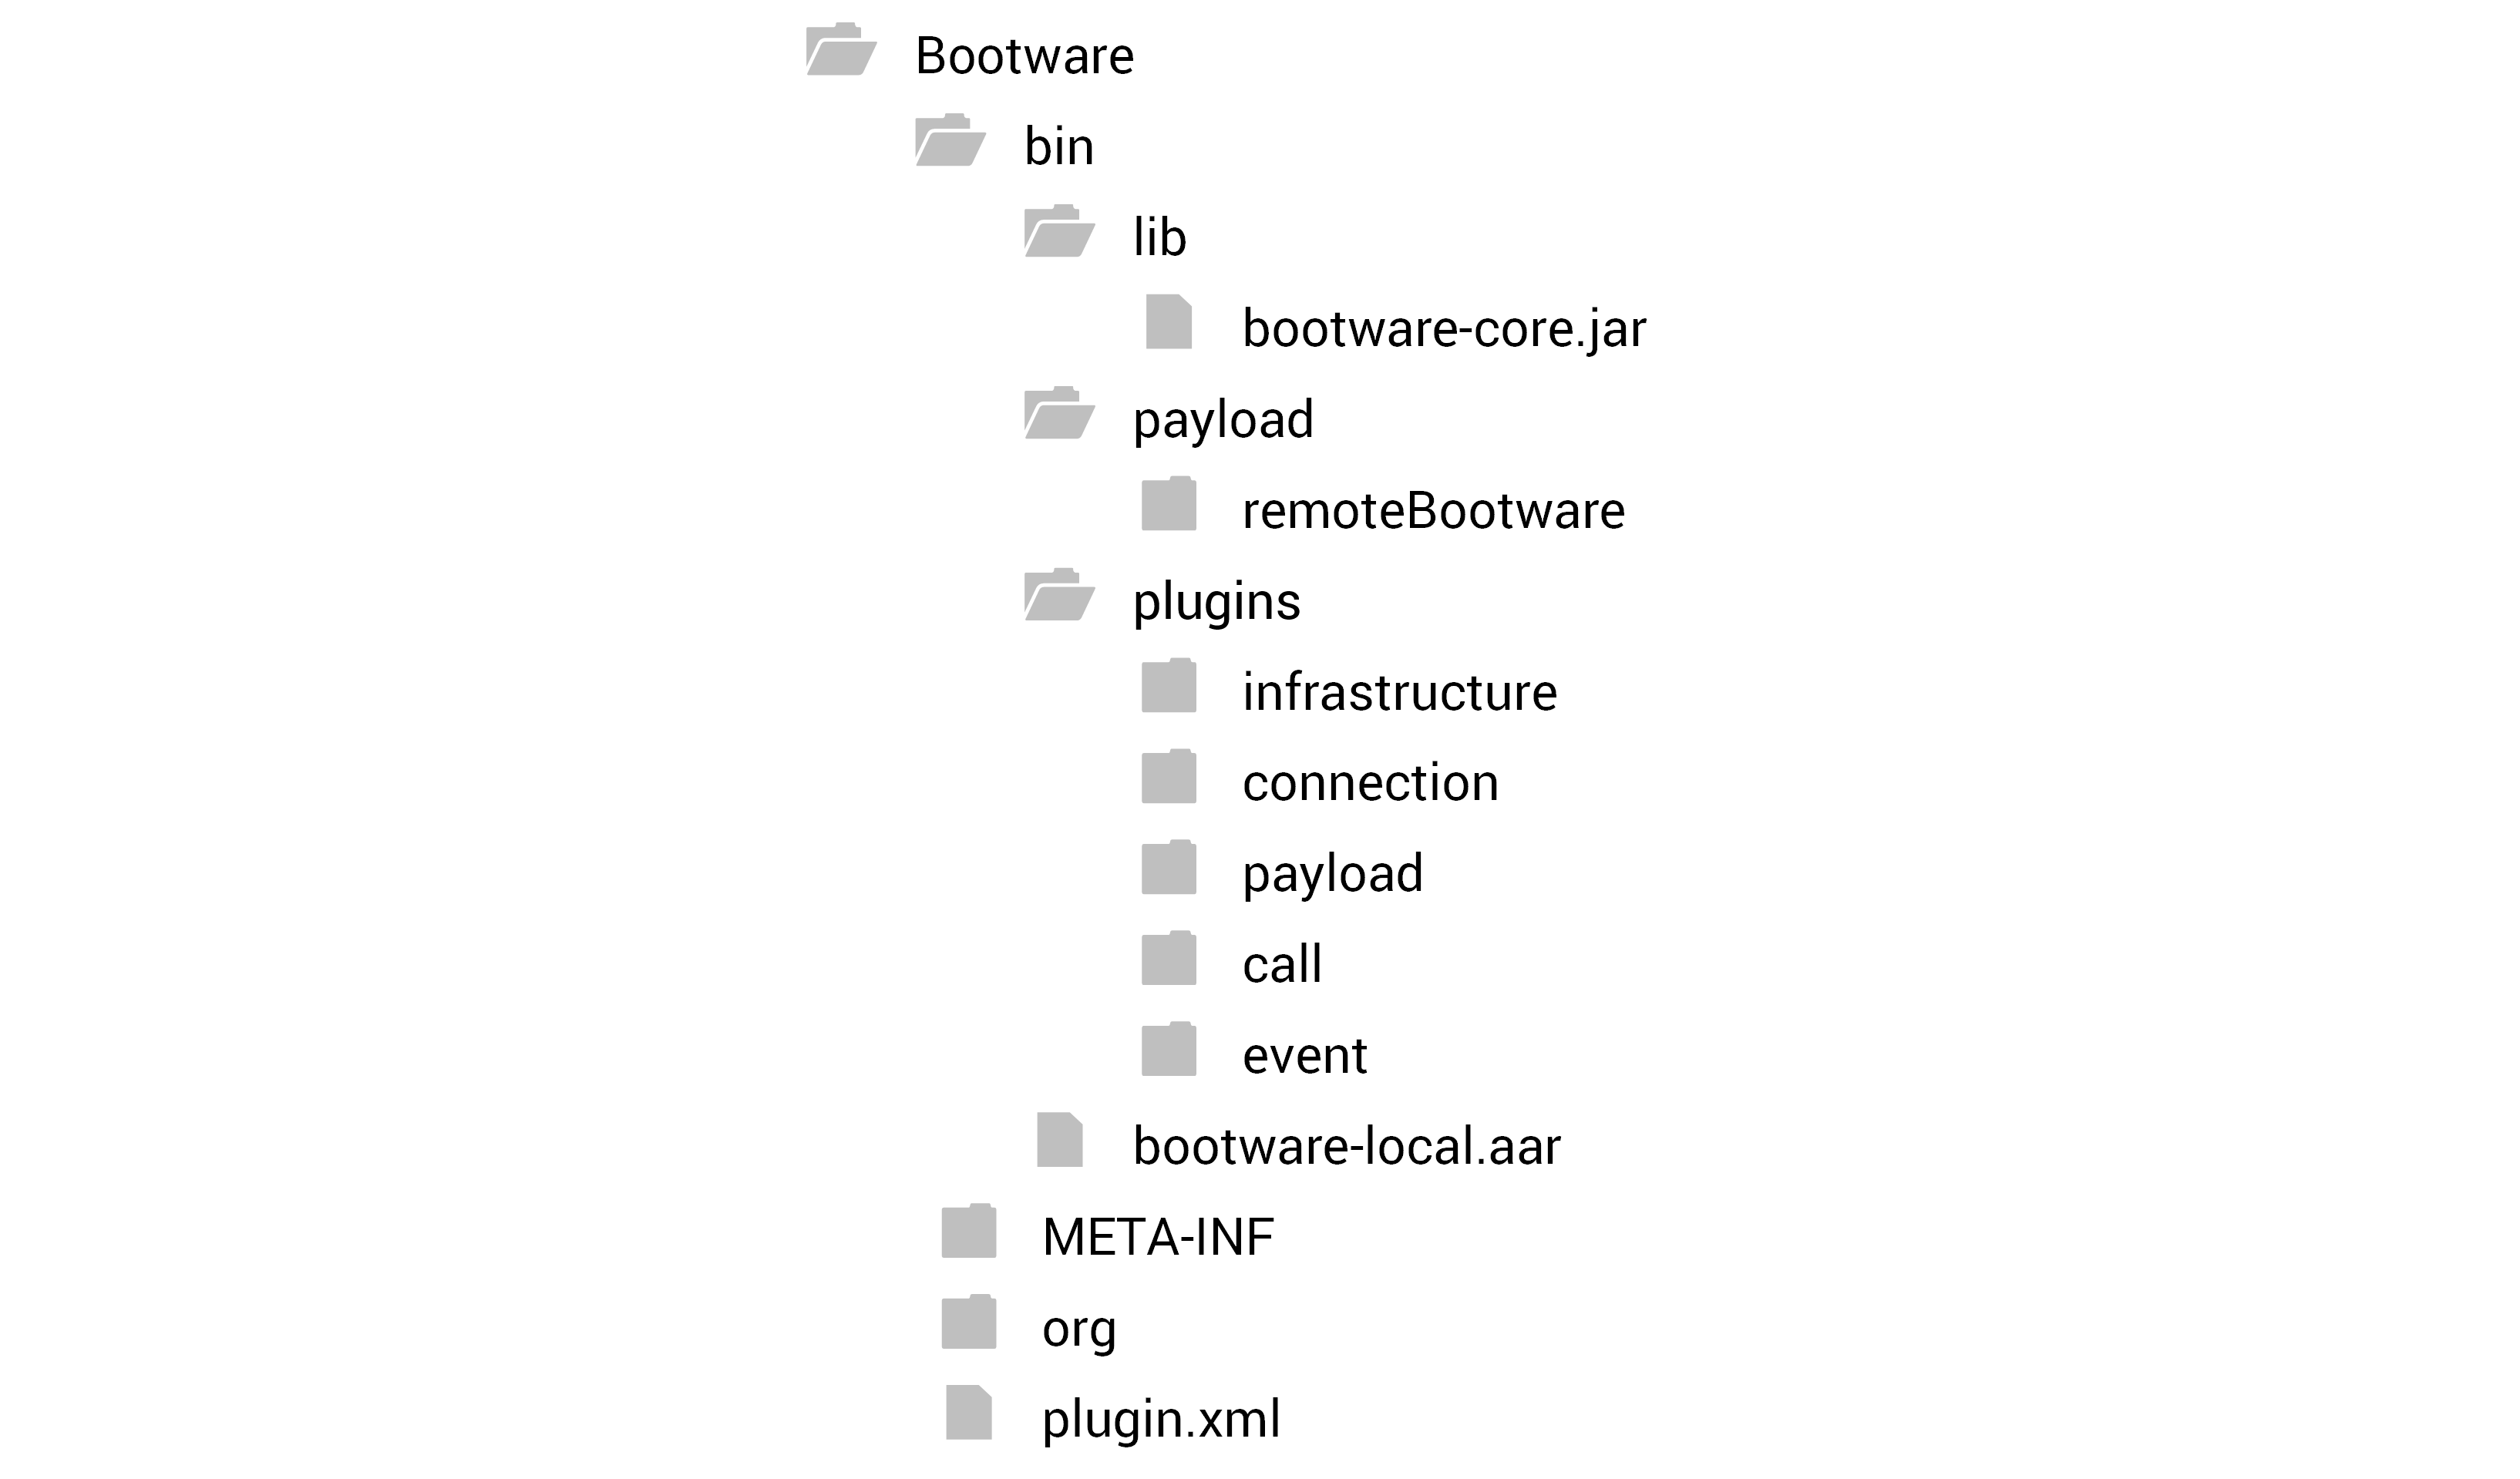
\includegraphics[resolution=600]{implementation/assets/packaging}
	\caption{The content of the bootware \textit{.zip} archive.}
	\label{imagepackaging}
\end{figure}

The bootware could be distributed in this format, but it is also possible to distribute a whole Eclipse directory that already contains the bootware plugin.
Either way, there are no other installation steps required then copying.
